% !TEX TS-program = pdflatexmk

\documentclass[runningheads, envcountsame, a4paper, draft, x11names]{llncs}
\usepackage{amsmath,amssymb,amsfonts}
\usepackage[scaled=0.8]{helvet}    % Less huge \textsf{functionName}
%\usepackage{enumitem}       % compacts lists and stuff
%\usepackage[subtle]{savetrees}
\usepackage[misc,geometry]{ifsym} % for letter symbol
\usepackage{soul}           % \hl for highlighting text; \st for strike-through
\usepackage{graphicx}
\usepackage[dvipsnames]{xcolor}
%\usepackage{wrapfig}
\usepackage{tikz}
\usetikzlibrary{trees,snakes,arrows}
\usetikzlibrary{shapes,chains}
\usetikzlibrary{positioning}
\usepackage{url}
\usepackage{hyperref}
\usepackage[nospace]{cite}

\usepackage[numbers, sort]{natbib}
\usepackage[T1]{fontenc} % E.g., for small caps in section headings
\usepackage{xspace}
\usepackage[lambda,advantage,operators,adversary,landau,probability,notions,logic,
ff,mm,primitives,events,complexity,asymptotics,sets,keys]{cryptocode}

% http://tug.ctan.org/tex-archkeIVe/macros/latex/contrib/todonotes/todonotes.pdf
\usepackage{todonotes}
\newcommand{\knote}[1]{\todo[inline,
                             color=orange,
                             size=\footnotesize
                         ]{\textsf{\textbf{Karl:} #1}}}
%\newcommand{\knote}[1]{}

% -- Fonts and styles for names
\newcommand{\mItemStyle}[1]{\ensuremath{#1}}
\newcommand{\mSetStyle}[1]{\ensuremath{\mathrm{\mathbf{#1}}}}
\newcommand{\mFunStyle}[1]{\text{\textup{\textsf{#1}}}}
\newcommand{\mConstStyle}[1]{\text{\textup{\textsf{#1}}}}
\newcommand{\mVarStyle}[1]{\mathit{#1}}
\newcommand{\mFactStyle}[1]{\text{\textsf{#1}}}
\newcommand{\mRuleStyle}[1]{\ensuremath{\mathbf{#1}}}
\newcommand{\mDomainStyle}[1]{\ensuremath{\mathcal{#1}}}



\begin{document}
\title{Formal Analysis of EDHOC Key Establishment for Constrained IoT Devices}
%
\author{Karl Norrman\inst{1,2}\textsuperscript{(\Letter)}\orcidID{0000-0003-0164-1478}
\and
Vaishnavi Sundararajan\inst{3}
\and
Alessandro Bruni\inst{4}
}
%
% Suggestion for shortened title in running heads:
%    Formal Analysis of EDHOC Key Establishment
%
%\authorrunning{K. Norrman et al.}
% First names are abbreviated in the running head.
% If there are more than two authors, 'et al.' is used.
%
\institute{
    KTH Royal Institute of Technology, Stockholm, Sweden \and
    Ericsson Research, Security, Stockholm, Sweden,\\
    \email{karl.norrman@ericsson.com} \and
    Ericsson Research, Int. Auton. Systems, Bangalore, India,\\
    \email{vaishnavi.sundararajan@ericsson.com} \and
    IT University of Copenhagen, Copenhagen, Denmark,\\
    \email{brun@itu.dk}
}
%
\maketitle
%

\begin{abstract}
%\hl{250 words}
IETF is standardizing an authenticated key establishment (AKE) protocol
named \mEdhoc{} for constrained IoT devices~\cite{selander-lake-edhoc-01}.
%
In contrast to more powerful devices like web cameras and cars, which receive a
lot of media attention, such devices operate under severe energy consumption
and message size restrictions.
%
\mEdhoc{} was first formally analyzed in 2018 by
Bruni~et~al.~\cite{DBLP:conf/secsr/BruniJPS18}.
%
Since then, the protocol has been significantly extended and now has three new
key establishment methods.
%
In this paper, we formally analyze all methods of \mEdhoc{} in a symbolic
Dolev-Yao model, using the \mTamarin{} verification tool.
%
We show that the different methods provide sensible, but also rather
heterogeneous security properties, and discuss various consequences of this.
%
Our work has also led to improvements in the design and the specification of
\mEdhoc.
%
\end{abstract}
%

% KARL: appears there are no standard keywords like in ACM and previous years
% SSR papers use very custom key words
\keywords{Formal verification \and Security \and IETF standardization \and
          Key establishment protocols \and Tamarin}

%-------------------------------------------------------------------------- sec
%\vspace{-2.5em}
\section{Introduction}
\label{sec:introduction}

%-------------------------------------------------------------------------- sub
\subsection{Background and motivation}
\label{sec:motivation}
IoT security threats involving computationally strong devices such as cars
and web-cameras receive the most attention from media and academia.
%
Securing communication between such devices can readily be done using existing
protocols like \mDandTls.
%
Constrained devices, on the other hand, which operate under severe bandwidth
and energy consumption restrictions, have received much less attention.
%
These devices may be simple sensors which only relay environment
measurements to a server every hour, but need to function autonomously without
maintenance for long periods of time.
%
To keep energy consumption down, highly specialized radio links with small
and heterogeneous frame sizes are sometimes used.
%
IETF defined the Constrained Application Protocol (\mCoap{}) protocol for data
transport in such situations~\cite{rfc7252}.
%
\mCoap{} does not include security protection on its own, and in some cases,
\mDandTls{} messages are too large to fit into the radio frames.
%
Thus, IETF standardized the Object Security for Constrained RESTful Environments
(\mOscore{}) protocol to secure communications between constrained
devices~\cite{rfc8613}.
%

The \mOscore{} protocol requires a pre-established security context.
%
For a couple of years, the IETF Lightweight Authenticated Key Exchange (LAKE)
working group has been developing requirements and mechanisms for a key
exchange protocol, named \mEdhoc~\cite{selander-lake-edhoc-01}, for
establishing \mOscore{} security contexts.
%
Naturally, \mEdhoc{} must work under the same constrained requirements as
\mOscore{} itself.
%
While use cases for \mEdhoc{} are not firmly set, the overall goal is to
establish an \mOscore{} security context, under message size limitations.
%

%-------------------------------------------------------------------------- sub
\subsection{Related Work}
\label{sec:relatedWork}
%
The first incarnation of \mEdhoc{} appeared in March 2016.
%
It contained two different key establishment methods, one based on a
pre-shared Diffie-Hellman (DH) cryptographic core and a second based on a
variant of challenge-response signatures, in the style of the \mNoise{}
framework~\cite{perrin2016noise}.
%
By a cryptographic core, or simply core, we mean an academic protocol, without
encodings or application specific details required by an industrial protocol.
%
By a key establishment method we mean a core with such details added.
%

The core based on challenge-response signatures was replaced by \mSigma{}
in May 2018.
%
Now, variants using challenge-response signatures have been added again by
integrating the cryptographic core of \mOptls{}.
%
Additionally, mixed variants where one party uses a challenge-response
signature and the other a regular signature have also been added.
%
Consequently, there are now five methods in total, and formal analysis is
required to verify security guarantees for \mEdhoc.
%
This is especially important, since the \mSpec{} itself lacks a description
of the intended security model and overall security goals.
%

Three cores have been analyzed in the computational model (\mSigma{}~\cite{DBLP:conf/crypto/CanettiK02},
\mOptls{}~\cite{DBLP:conf/eurosp/KrawczykW16}, and
\mNoise{}~\cite{DBLP:conf/eurosp/KobeissiNB19}).
%
However, there are significant departures from these cores in \mEdhoc, and
these proofs do not carry over automatically
(See Section~\ref{sec:relationsToOtherProtocols}).
%
The work closest to ours is Bruni~et~al.~\cite{DBLP:conf/secsr/BruniJPS18},
formally analyzing the May 2018 version of \mEdhoc{} (with two methods) in
\mProverif~\cite{DBLP:conf/csfw/Blanchet01}.
%

%\knote{should be moved to section 3}
%
%Computational models often rely on implicit session key authentication
%(see, for example, the definition of SK-security in the Canetti-Krawczyk
%model~\cite{DBLP:conf/crypto/CanettiK02}).
%%
%Although symbolic models predominantly rely on correspondence properties
%in the style of Lowe~\cite{DBLP:conf/csfw/Lowe97a}, there are examples where
%implicit session key authentication has been used.
%%
%For example, Schmidt~et~al.~\cite{DBLP:conf/csfw/SchmidtMCB12} use a
%symbolized version of an extended Canetti-Krawzcyk model.
%%

%-------------------------------------------------------------------------- sub
\subsection{Contributions}
\label{sec:contributions}
We formally analyze the \mEdhoc{} protocol in the \mTamarin{}
tool~\cite{DBLP:conf/cav/MeierSCB13}.
%
This work is presented in Section~\ref{sec:formalization}.
%
The formal models and proven properties are based on the version as on
2020-03-01~\cite{selander-lake-edhoc-01}.
%
We give an explicit security model for the protocol and verify essential
properties, such as session key and entity authentication and perfect forward
secrecy, for all five methods.
%
We also discuss the relationship between proven properties and the claimed
security properties, and the lack of a precise security model for \mEdhoc{}.
%
In fact, the standard has already been improved based on our analysis,
which we discuss in Section~\ref{sec:discussion}.
%

%-------------------------------------------------------------------------- sec
\section{The \mEdhoc{} Protocol}
\label{sec:edhoc}
% !TEX root =  main.tex

%Description of \m\mEdhoc and main changes from last verified version

\vnote{Note for discussion with others: I find the macros for the protocol, method, and tool names distracting while reading through (the font changes too much, too often). The macro for EDHOC actually inserts a line break if you start a sentence with it, because of the \texttt{hbox} (I'm not sure why the hbox exists for what is a macro to be inserted in running text). I do need to start sentence with EDHOC many times though, so this is irritating. It is also the case that ProVerif needs to be written like so, and not capitalized entirely, so at least one of them is plain wrong! For now I've left in the macros, but I'd prefer that we fixed them to be regular capitalized text or, in the case of ProVerif, in camelcase as they should be.}

\vnote{Macros don't work right in section headers!}

\subsection{Overview}
Constrained IoT systems often deal with a lot of valuable personal and business information that ought to be kept secure. Such systems need to be assured of end-to-end protection with source authentication and perfect forward secrecy. It is often desirable to protect such devices at the application layer -- for example, in cases where transport layer security is not sufficient [\mcneed], or where multiple underlying protocols need to be accounted for. One method for providing application layer security is provided by CBOR Object Signing and Encryption (\mCose) [RFC8152: \mcfix].  

In order to derive shared key material with which to proceed, communicating parties can run an Elliptic Curve Diffie-Hellman key exchange protocol with ephemeral keys. Ephemeral Diffie-Hellman Over \mCose (\mEdhoc) is a lightweight key exchange protocol for such situations, and is expected to provide perfect forward secrecy and identity protection. \mEdhoc supports authentication using pre-shared keys (PSK), raw public keys (RPK), and public key certificates. After successful completion of the \mEdhoc protocol, application keys and other application specific data can be derived using the \mEdhoc-Exporter interface. 

A main use case for \mEdhoc is to establish a security context for Object Security for Constrained RESTful Environments (\mOscore) [RFC8613: \mcfix]. \mOscore is a protocol which uses \mCose for application-layer protection on top of the transport-layer Constrained Application Protocol (CoAP). \mEdhoc uses \mCose for cryptography, CBOR for encoding, and CoAP for transport. By reusing existing libraries, the additional code footprint can be kept very low.

\mEdhoc is designed to work in highly constrained scenarios. This makes it especially suitable for network technologies which have low throughput, low power consumption, and small frame sizes. Examples include Cellular IoT, 6TiSCH, and LoRaWAN [\mcneed].

The \mEdhoc protocol can establish Diffie-Hellman key exchange in one of three different ways -- using digital signatures, static Diffie-Hellman (DH) keys, or pre-shared symmetric keys. We describe each of these methods in detail below. The communicating parties must agree on the method and cipher suite used for encryption as part of the first message. The parties exchange ephemeral public keys, compute the shared secret, and derive symmetric application keys from this secret.

The \mSigma (SIGn-and-MAc) family of protocols [\mcneed] has many variants. The \mSig-based methods of \mEdhoc are built on \mSigmaI, a variant of the \mSigma protocol which provides identity protection for the initiator, and  implements the \mSigmaI variant as Mac-then-Sign. The method involving static DH keys proceeds along the lines of \mOptls, with the agent creating a MAC and encrypting it using an algorithm for authenticated encryption with associated data (\mAead) [\mcneed]. 

\mEdhoc allows the initiator and responder to run different methods, combining \mSig and \mStat -- for example, the initiator might run a \mSig-based method, while the responder is running a \mStat-based method. This set of methods is not covered in previous versions of \mEdhoc, which only had a single \mSigma asymmetric key method (corresponding to the \mSigSig method shown in Section~\ref{sec:methods}). This allows one party to use a \mSigma style of authentication using signatures, while the other can use static DH keys. In Figure~\ref{fig:edhocasym}, a template for all the asymmetric key methods of EDHOC is shown. 

\begin{figure}[!h]\label{fig:edhocasym}
\centering
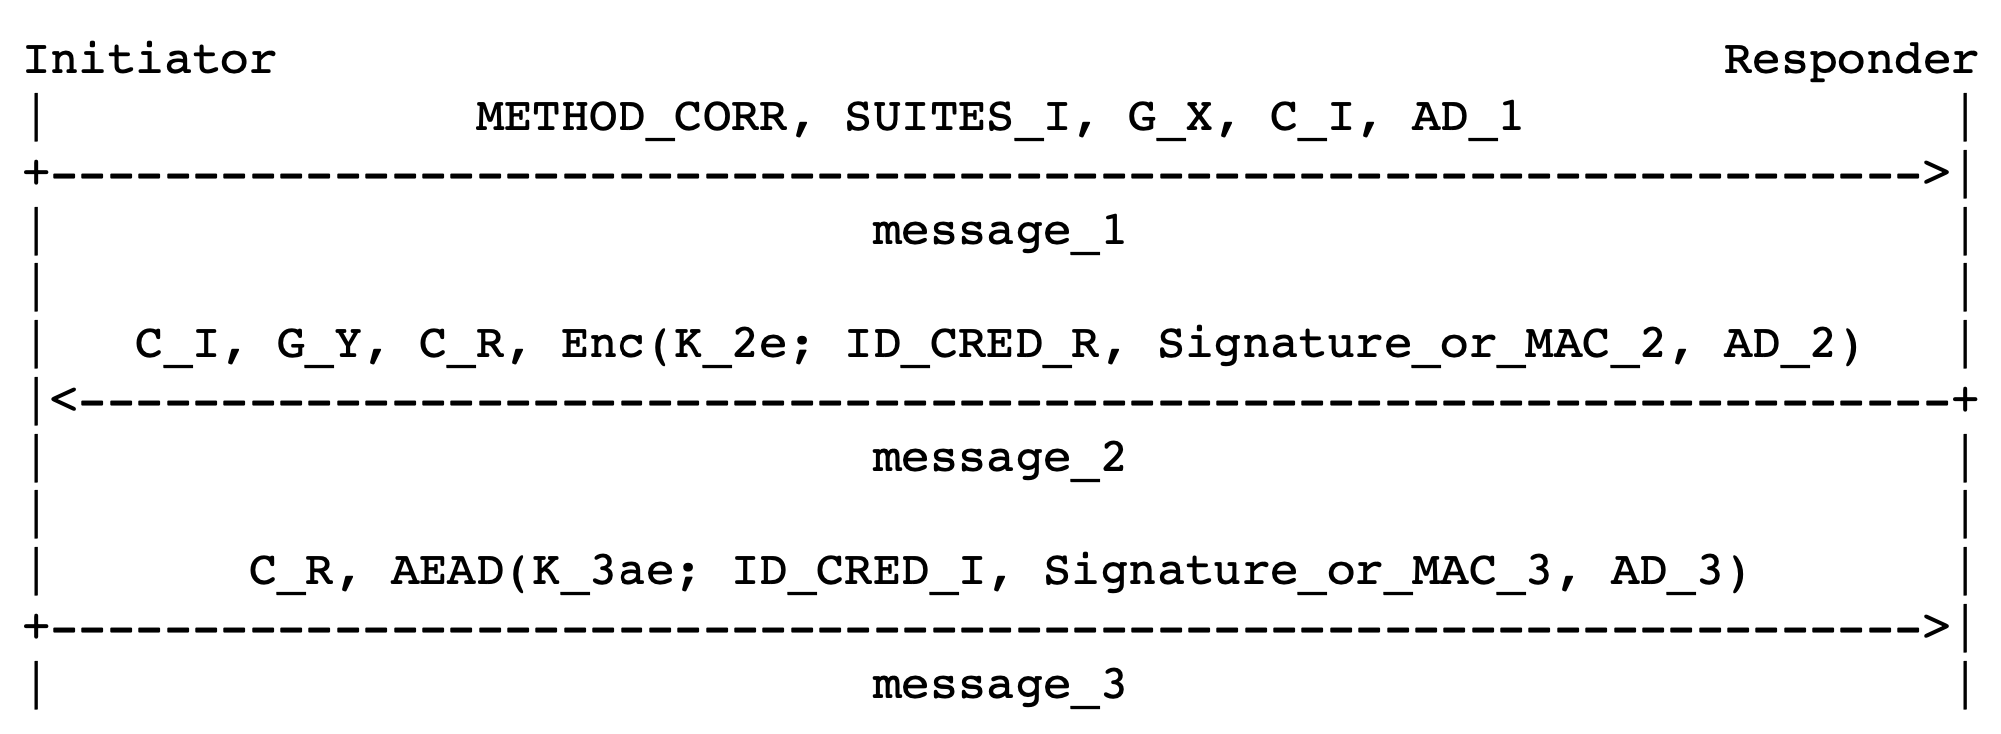
\includegraphics[scale=0.3]{Images/asym.png}
\caption{A template for the asymmetric key methods of EDHOC}
\end{figure}

\subsection{Background, comparison with~\cite{DBLP:conf/secsr/BruniJPS18}}
The first version of \mEdhoc was proposed in March 2016 to a working group investigating lightweight authenticated key exchange protocols [\mcneed]. There has been a focus on formally verifying that the protocol satisfies the properties expected of it right from the beginning. 

The 2018 work~\cite{DBLP:conf/secsr/BruniJPS18} by Bruni et al performed a formal verification of version 08 [\url{https://tools.ietf.org/html/draft-selander-ace-cose-ecdhe-08} \mcfix] of \mEdhoc. The protocol and properties are modelled and verified in the \mProverif tool. This version of the protocol belongs to the \mSigmaI family of protocols, and has two modes -- one with asymmetric keys, and one with pre-shared symmetric keys (PSK). Bruni et al showed that this version satisfies the requisite properties of identity protection, (perfect forward) secrecy of data, and strong authentication, upon completion of the protocol.

\mEdhoc has undergone a lot of change since version 08, as will be described in the following sections, and the formal verification of the current version, therefore, is a worthwhile exercise.

\subsection{Comparison with \mOptls and \mNoise}
\vnote{Would this perhaps be better served by putting it in related work?}


\section{Methods and features of \mEdhoc}\label{sec:methods}

\subsection{Fundamental components of \mEdhoc}
\subsubsection{\mCose}
\mCbor is a data format designed for small code size and small message size. The \mCbor Object Signing and Encryption (\mCose) protocol is used to create and process signatures, MACs, and encryption using CBOR. 

A \mCose object contains bitstrings corresponding to protected parameters (which ought to be cryptographically protected), unprotected parameter, and the payload to be signed. This can be signed/encrypted/MACed, to obtain a resultant \mCose object containing the bitstring corresponding to the operation. The respective algorithms may also be fed some externally supplied data, which is carried along with the \mCose object, but is not part of it. \mEdhoc only uses the signature and encryption objects of \mCose. For encryptions, \mCose supports two different methods -- one where the recipient is not needed because the key is known implicitly, and one for all other cases. \mEdhoc only uses the former. 

A \mCoseEncrypt structure as used in \mEdhoc is a \mCbor array with a text field which contains the string ``Encrypt0'' to denote the use of the method with implicit recipient, a field for protected data, a field for externally supplied application data, and a field for ciphertext. All these fields store the corresponding bitstrings.

\subsubsection{\mAead}
Authenticated encryption with associated data, or \mAead, is an authenticated encryption operation. The algorithm takes in a key, a unique nonce, a plaintext, and some associated data, and outputs a ciphertext. The plaintext is both authenticated and encrypted, while the associated data is merely authenticated. The ciphertext is at least as long as the plaintext. When the plaintext is empty, the \mAead algorithm acts as a MAC on the associated data. 

The associated data is used to protect information that needs to be authenticated, but does not need to be kept confidential. It might be desirable to authenticate this information, although it must be left unencrypted to allow the system to function properly. Authentication is provided without copying the data into the plaintext.

\subsubsection{Key derivation function (KDF)}
Perhaps the most important building block for \mEdhoc is the key derivation function based on \mHkdf [\mcneed], which is used to generate the pseudorandom strings and keys for the encryption operations in the communicated messages. The pseudorandom strings (\mPRKtwo and \mPRKthree) are derived using the \mHkdf-Extract function, while the keys are generated using the \mHkdf-Expand function. Both these functions are based on \mHmac [\mcneed], which is a hashing system for message authentication.

The \mHkdf-Extract function is run with a salt and some input keying material (IKM) as input. It produces as output a pseudorandom string. For the \mPskPsk method alone, the salt is the key pre-shared between the initiator and the responder, while for the other methods, it is empty. The IKM for all \mEdhoc methods is the ECDH shared secret \mGxy.

In order to generate keys for the various encryptions, the \mHkdf-Expand function is used. This is run with a pseudorandom string, an info string, and the length of the output keying material (OKM) as input. The pseudorandom string is generated using \mHkdf-Extract as above. The info string contains details of the \mAead encryption algorithm used, length of the OKM, and the transaction hash as used for the specific method (a detailed discussion follows, for each method). In case the length $l$ of the OKM is shorter than that of the transaction hash, the OKM is obtained by taking the first $l$ bits of the result of running \mHmac on the pseudorandom string, and a concatenation of 0x01 and the info strings.

We now discuss each of the \mEdhoc methods in detail in the next few sections.

\subsection{\mPskPsk method}
In this method, the initiator and responder are assumed to have a pre-shared key which is secret to them, and can be retrieved by the responder using a public part of the first message (\mIDPSK). This method corresponds to the symmetric key method of \mEdhoc v08. 

In the first message, the initiator sends a message consisting of the method name, the cipher suites ranked in order of preference, the initiator's ephemeral key (\mGx), their connection identifier (\mCi), the \mIDPSK identifier, and (optional) auxiliary data (\mADone). The responder, upon receipt of this message, must verify that the selected cipher suite is supported,  and pass \mADone to the security application which needs it. If any verification step fails, the initiator sends an EDHOC error message back, and the protocol aborts.

The second message, sent by the responder, is composed of \mCi, the responder's ephemeral key \mGy, their connection identifier \mCr, and a \mCose object. This contains as external data the transaction hash of the first message (\mTHtwo), along with an \mAead encryption of the (optional) auxiliary data \mADtwo. The key used for this (\mKtwo) is derived using the EDHOC key derivation function with \mTHtwo and the pseudorandom string \mPRKtwo as input, while the associated data for the \mAead encryption is constructed by concatenating a constant string, plaintext \mhplain, and \mTHtwo. Recall that \mPRKtwo is constructed by running \mHkdf-Extract using the pre-shared key as salt. 

The initiator, upon receipt of this message, sends back \mCr, followed by a \mCose object containing an \mAead encryption of auxiliary data \mADthree, along with the transaction hash of the second message (\mTHthree) as external data. As earlier, the key used is derived by supplying \mTHthree and \mPRKthree as input to the KDF, and the associated data obtained by concatenating the constant string, plaintext \mhplain, and \mTHthree. An abstract description is shown in Figure~\ref{fig:edhocpsk}.

\vnote{Figure numbers don't square up, check class file guidelines!}

\begin{figure}[!h]\label{fig:edhocpsk}
\centering
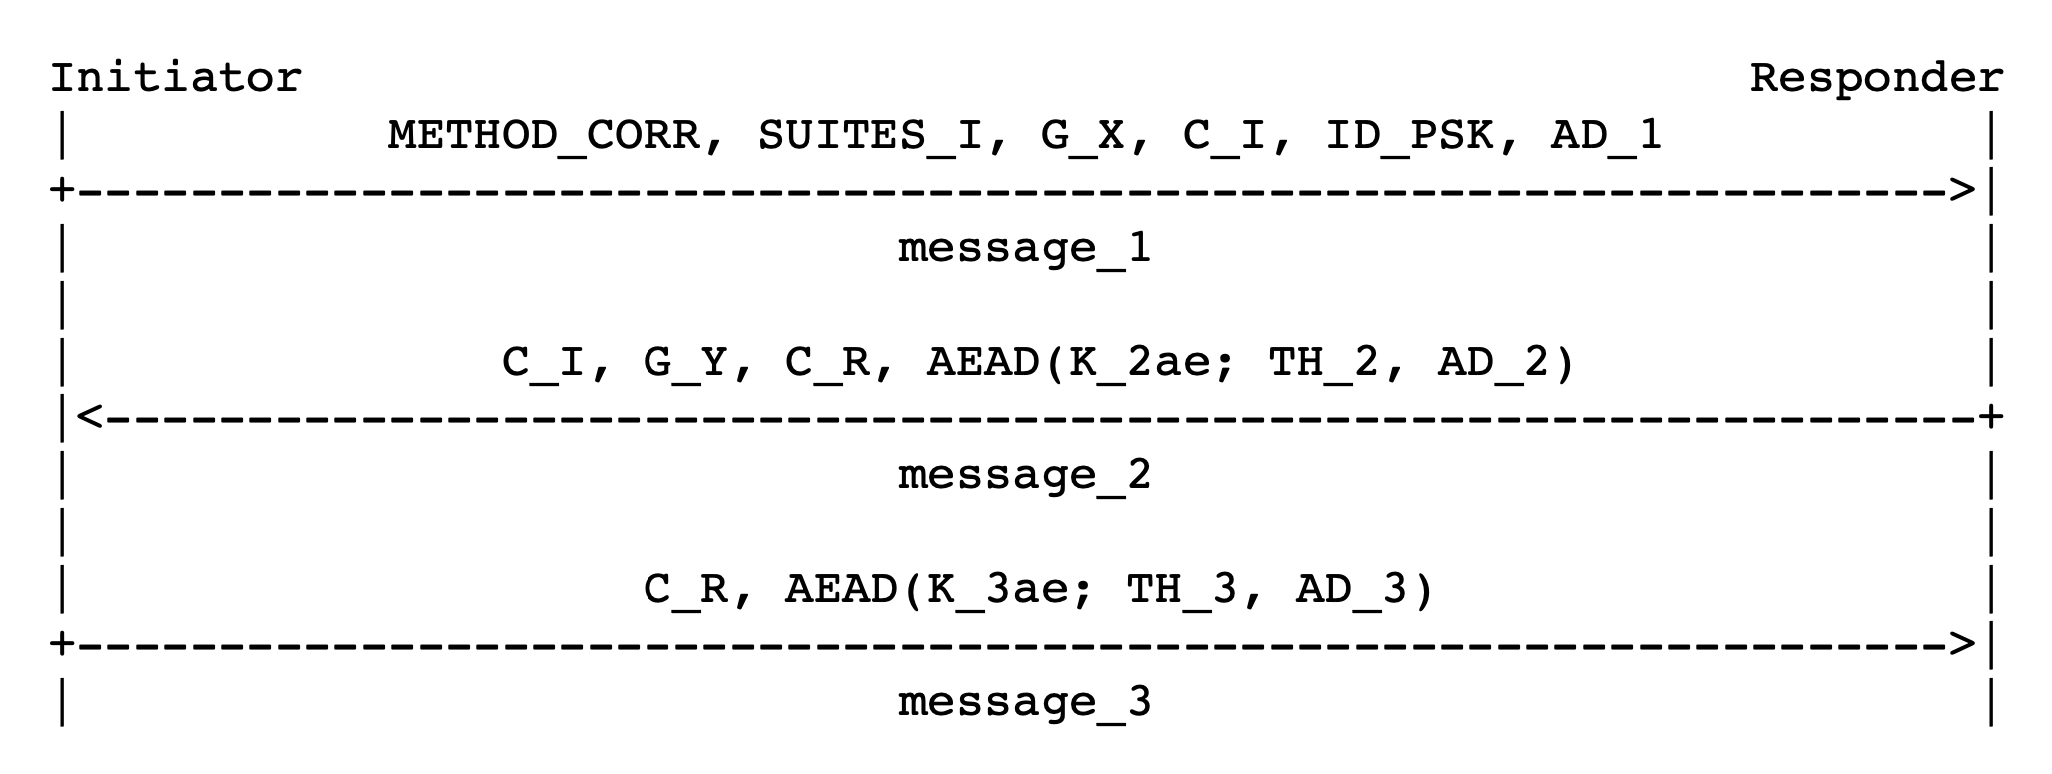
\includegraphics[scale=0.3]{Images/psk.png}
\caption{The PSK-PSK method of EDHOC}
\end{figure}

\subsection{\mStat-based methods}
\mEdhoc allows for three \mStat-based methods -- two where only one participant has a static Diffie-Hellman key (while the other uses signatures), and one where both do. 

In the first message, the initiator includes an identifier for the method, a preference-ordered list of cipher suites, their ephemeral key \mGx, their connection identifier \mCi, and some optional plaintext \mADone. This message is common to all the four methods below involving asymmetric keys. 

The responder, upon receipt, verifies the cipher suites, passes any \mADone to the application that needs it, and proceeds to construct and send the second message. This message contains (not necessarily all of) \mCi, \mGy, \mCr, and an encrypted term. The initiator, upon getting this message, sends out a message containing an encrypted term. Depending on the methods being run by the initiator and responder, the exact contents of these messages may vary. We will now describe each of these methods and the second and third messages therein in detail.

\subsubsection{\mSigStat}
The initiator runs a \mSigma-based method, with signatures, while the responder operates with a static Diffie-Hellman key and MACs. Since this method is one where the responder runs \mStat, in the second message, \mCi is omitted. The encrypted term for the second message is constructed as follows. 

First, we build the \mCose object that is the inner MAC, since the responder runs \mStat. The protected part of this object is an identifier for retrieving the responder's public authentication key \mCredr. The externally supplied data is the transaction hash \mTHtwo of the first message and \mGy,  the responder's public authentication key \mCredr, and (optional) auxiliary data \mADtwo. The key used for the encryption is the output of the KDF on being fed as input the pseudorandom string \mPRKthree and \mTHtwo. The resulting encrypted object is now referred to as the ciphertext \mMactwo. 

For the outer encryption object, we consider the plaintext formed by concatenating the bitstrings corresponding to the identifier for \mCredr, \mMactwo, and \mADtwo (if any). The encryption is obtained by performing an \mXor operation on this plaintext with the key \mKtwo, which is obtained by using the KDF on \mPRKtwo and the transaction hash \mTHtwo. The responder therefore sends to the initiator \mGy, \mCr, and this \mCose encryption object as the second message.

The initiator responds with the third message, consisting of \mCr, and an encrypted object. Here, again, we first build the inner \mCose object. This process is analogous to that employed by the responder for the second message. The \mCose object has as protected data an identifier for retrieving the initiator's public authentication key \mCredi. The externally supplied data is the transaction hash \mTHthree of the second message and \mTHtwo,  the initator's public authentication key \mCredi, and (optional) auxiliary data \mADthree. The key used is obtained by inputing the pseudorandom string \mPRKfour and \mTHthree. The resulting encrypted object is now referred to as the ciphertext \mMacthree. 

Since the initiator is running \mSig, this \mCose object needs to be signed. To the signing algorithm, the initiator sends as protected data the identifier for retrieving \mCredi, as external data the concatenation of \mTHthree, \mCredi, and any \mADthree, and the payload \mMacthree. This is signed using the private authentication key of the Initiator.  

We now construct the encryption for the third message, by passing to an \mAead encryption algorithm a \mCose object with no protected data, external data \mTHthree, and a plaintext obtained by concatenating the identifier for retrieving \mCredi, the signed object described above, and \mADthree. The key used for encryption is \mKthree, obtained by running the KDF on the pseudorandom string \mPRKthree and \mTHthree. Thus, the message sent by the initiator to the responder in the third step is \mCr accompanied by this encrypted object.

\subsubsection{\mStatStat}
In this method, both the initiator and the responder run the \mStat method. The responder's message looks exactly the same as in the previous subsection, for \mSigStat. The initiator's message, however, is not signed anymore, since the initiator too is running the \mStat method. Thus, we skip the signature process in the steps described above, and instead of passing a signed object to the \mAead encryption algorithm, we pass \mMacthree itself. Everything else stays the same as earlier.

\subsubsection{\mStatSig}
Here, the responder runs the \mSig method, while the initiator runs the \mStat method. Thus, the second message, sent by the responder to the initiator needs an extra layer of signing. Once \mMactwo has been constructed, as in the methods where the responder runs \mStat, the responder runs the signature algorithm with a \mCose object. This object has the identifier for \mCredr as protected data, a concatenation of \mTHtwo, \mCredr, and \mADtwo as external data, and the payload \mMactwo. This is signed using the responder's private authentication key.

The outer encryption object is constructed by considering a plaintext consisting of \mCredr, this signed object (instead of \mMactwo, as was the case when the responder ran the \mStat method), and \mADtwo. \mKtwo is generated the same way as earlier, and the responder sends \mGy, \mCr, and this encrypted object to the initiator as the second message.

Since the initiator is running the \mStat method, there is no change in the third message from the previous case. There is no signature, and only \mMacthree is encrypted via \mAead.

\subsection{\mSigSig method}
In this method, both parties run the \mSig method, and therefore, both the second and third messages need to be signed before being encrypted via \mAead. The second message looks like the one from the \mSigStat method described above, while the third looks like the one from the \mStatSig method.


\vnote{Need to insert tikZ figures}

\subsection{Deriving an OSCORE context}
\mEdhoc is often used to set up parameters for \mOscore. In this case, the parties make sure that the connection identifiers are distinct, i.e. $\mCredi \neq \mCredr$, since these are used as \mOscore sender IDs. If the initiator plays the role of the CoAP client, and the responder the role of the CoAP server, the client gets the sender ID \mCredr and the server the ID \mCredi (the identifiers are swapped). The \mAead and hash algorithms for \mOscore stay the same as those used for the selected cipher suite in \mEdhoc, while the master secret for \mOscore is derived using the key length of the \mAead algorithm of \mEdhoc. 

\subsection{Expected security properties}



%-------------------------------------------------------------------------- sec
\section{Formalization and Results}
\label{sec:formalization}
% !TEX root =  main.tex
 
Next we describe our approach towards formalizing the \mEdhoc{} protocol. We use the
symbolic (Dolev-Yao) model for verification, with \mTamarin{} for tool support.
%
The next three subsections describe our threat model, briefly present the
\mTamarin{} tool, and our modeling choices.
%
Finally, we present the properties that we proved in this effort.

 
\subsection{Threat Model}\label{sec:threat-model}
 
We verify \mEdhoc{} in the symbolic Dolev-Yao model: as customary in this style of
modeling, we assume all cryptographic primitives to be ``perfect'', and hence
only allow the attacker to encrypt and decrypt messages when they know the key,
and exclude hash collisions, for example; the attacker is in control of the
communication channel, and can interact with unbounded sessions of the protocol,
dropping, injecting and modifying messages at their liking.

One important point of the modeling is that we allow the attacker to impersonate
dishonest and/or compromised endpoints, by revealing their long-term and session
key material at any given point.
%
Conversely, we say that a party is honest if they never reveal their
long-term key or session key material.

Another important point is to define what the key material is.
    \mEdhoc{} does not result in an explicit session key, but a cryptographic
    state from which keys for \mOscore{} can be derived using \mHkdf.
    As will be seen below, depending on how the key material is defined, the
    different methods will have different authentication properties.
    In particular, all methods except those where the initiator uses the
    \mStat{} method provide a stronger form of authentication (injective
    agreement) for the initator.

 
\subsection{Desired Properties}
\label{sec:desired-properties}
 
Next we list the properties that will be considered during verification.
\knote{The title should be "verified properties" or "considered properties" or
    similar. "desired" requires us to specify who think they are desired and
    give rationale for why the are desired.  Also, one of the points of the
    paper is that without more specific goals for EDHOC, it is not clear what
constitutes desirable.}

 
\subsubsection{Secrecy}
\knote{Please add a dot at the end of all subsubsections and paragraphs (llncs
guidelines)}
We say that \mEdhoc{} satisfies secrecy of the established session key $sk$
between two honest parties $A$ and $B$ if, for any run of the protocol $A$ and
$B$, the attacker does not get to know $sk$.
%
The attacker may passively observe---and actively interfere with---the
communication, and run any number of sessions with $A$ and $B$, in either role,
concurrently or otherwise.

 
\subsubsection{Authentication}
To define \mEdhoc{}'s authentication properties we make use of Lowe's definition
of \emph{injective agreement}~\cite{DBLP:conf/csfw/Lowe97a}:
\knote{Maybe we don't need to quote the definition and could paraphrase it in a
shorter form to save space.}
\begin{quote}
  ``We say that a protocol guarantees to an initiator $A$ [injective] agreement
  with a responder $B$ on a set of data items $ds$ if, whenever $A$ (acting as
  initiator) completes a run of the protocol, apparently with responder $B$,
  then $B$ has previously been running the protocol, apparently with $A$, and
  $B$ was acting as responder in his run, and the two agents agreed on the data
  values corresponding to all the variables in $ds$, and each such run of $A$
  corresponds to a unique run of $B$.''
\end{quote}
%
We say that \mEdhoc{} in method $m$ satisfies \emph{explicit authentication} for
the initiator $A$ with a responder $B$, if injective agreement holds for $A$
with $B$ on the session key $sk$, when running method $m$.
%
The corresponding definition for the responder is analogous.
%
If both parties obtain explicit authentication we refer to it as mutual explicit
authentication or simply explicit authentication when it is clear from the
context.

A party obtains the explicit authentication guarantee when both parties agree
on the session key (and other parameters), when the party completes the protocol
run.
%
It turned out, however, that explicit authentication does not hold for all
\mEdhoc{} methods, in which cases we prove \emph{implicit authentication} as
defined in~\cite{DBLP:journals/iacr/GuilhemFW19}.
%
In a nutshell, a protocol satisfies \emph{implicit authentication} if the
initiator and responder agree on the session key \emph{only after} a successful
execution of the protocol.
%
That is, authentication happens only implicitly, as there is no confirmation to
the initiator that the responder has computed the same session key.
%
More precisely, we adapt the definition of~\cite{DBLP:journals/iacr/GuilhemFW19}
to the symbolic model, and we prove that if an initiator $A$ and a responder $B$
complete the protocol deriving the same session key, then $A$ believes she is
talking to $B$ and $B$ believes he is talking to $A$.

 
\subsubsection{Session Independence}
A protocol satisfies session independence if knowing a session key does
not give the attacker any information about other sessions.  To model session
key independence of \mEdhoc, we allow leakage of session keys, and additionally
check security only of those sessions for which the session keys have not been
directly revealed to the attacker.

 
\subsubsection{Perfect Forward Secrecy} (PFS) A protocol satisfies perfect forward
secrecy if, for any run of the protocol in which the initiator and the responder
agree on a session key $sk$, the attacker does not learn $sk$, even when the
long-term keys are revealed after the session is completed.

 
\subsubsection{Key-Compromise Impersonation} (KCI) This property takes the perspective of one
of the endpoints of the protocol, say Alice running a session with Bob. A
protocol is secure under KCI if Alice can still establish a secure session with
Bob, even though Alice's keys are compromised at any time, and Bob's key
material is not leaked until the end of the session.

 
\subsubsection{Post-Compromise Security} (PCS) A protocol that has
\emph{post-compromise security} (following definitions in~\cite{cohn2016post})
is capable of establishing a secure session even after one of the parties has
been compromised. Cohn-Cordon et al.~\cite{cohn2016post} presents two notions of
PCS, namely weak and strong PCS: here we focus on the latter.
%
A protocol guarantees \emph{weak PCS} if secrecy of any session key $sk$ holds
between the initiator and the responder, even if the run of the protocol that
established $sk$ happens after a \emph{limited compromise}, where the key
material is not leaked, but the attacker is capable of impersonating both
parties (i.e. has the ability to perform all cryptographic operations using the
initiator's and responder's long term keys, but has not access to the long term
keys).

 
\subsection{\mTamarin{}}
\label{sec:tamarin}
 
We chose \mTamarin{} to model and verify \mEdhoc{} in the Symbolic model.
%
\mTamarin{} is an interactive verification tool based on multi-set rewriting rules
with event annotations, which allows the user to check Linear Temporal Logic
(LTL) formulas on these models.
%
Multi-set rewrite rules with events take the form $ l \ifarrow[e] r $,
where $l$ and $r$ are multi-sets of facts, and $e$ is a multi-set of events.
Facts are $n$-ary predicates over a term algebra, which defines a set of function
symbols $\mathcal F$, variables $\mathcal V$ and names $\mathcal N$. \mTamarin{}
checks equality of these terms under an equational theory $E$. For example,
one can write $ dec(enc(x,y),y) =_E x $
to denote that symmetric decryption reverses the encryption operation under this theory.
All operations on terms are defined under $E$, hence we omit the
subscript from now on as the equational theory is fixed per model.

 
\subsubsection{Semantics and Built-ins} \phantom{} \mTamarin{} states
$S$, $S'$ are multisets of facts, and a semantic transition $S \semarrow[E] S'$
occurs if there is a rule $l \ifarrow[e] r$ and a substitution $\sigma$ such
that $S \supseteq \sigma(l)$ and $S' = S \setminus \sigma(l) \uplus \sigma(r)$
and $E = \sigma(e)$.

There are a few more details, such as persistent facts that are denoted by a $!$
and are never removed from the state.
%
The sorts fresh (denoted by $\sim$) and public (denoted by $\$$) denote fresh
constants and public values known to the attacker respectively, and are both
sub-sorts of a base sort.
%
Finally, \mTamarin{} has some built-in predicates ($\mIn,
\mOut$ to represent input and output of messages with the attacker,
and
$\mFr$ to denote a fresh constant created in the current rule, among
others), rules and equations that represent the attacker's knowledge
and standard equational theories in the symbolic model,
which we present later.

\anote{This can go, I make a shorter note later:\\
{Notational conventions} In the remainder of this section we present
\mTamarin{} code as it appears in the models that we verify, in the style of
literate programming.  Whenever possible we match the style of the protocol
diagrams in Section~\ref{sec:edhoc} and the naming convention of the \mEdhoc{}
\mSpec~\cite{selander-lake-edhoc-01}, so that each element of the model is
traceable to the standard.  There are a few exceptions to this, most notably
some variable names that we introduce for the sake of the \mTamarin{} model and are
not present in the original \mSpec{}, which will appear in \mT{camelCase}, and
the syntax for Diffie-Hellman exponentiation which is specific to \mTamarin{}.
We also use \mT{xx} to name the ephemeral key for the initiator (resp. \mT{yy}
for the responder) as to avoid confusion with \mTamarin's builtin variable
names \mT{x} and \mT{y}.}

 
\subsubsection{Protocol Rules and Equations}
\mTamarin{} allows users to define new function symbols and equational theories.
These user defined objects are then translated by \mTamarin{} into rewrite
rules, which are added to the set of considered rules during verification.
For example, in our model we have a symbol to denote authenticated encryption and
hence \mTamarin{} produces the rule:
%
\begin{lstlisting}
[!KU(k), !KU(m), !KU(ad), !KU(al)] --> [!KU(aeadEncrypt(k, m, ad, al))]
\end{lstlisting}
%
to denote that if the attacker knows a key \mT{k}, a message \mT{m}, the
authenticated data \mT{ad}, and an algorithm \mT{al}, then they can construct
the encryption using these parameters, hence get to know the message
\lstinline{aeadEncrypt(k, m, ad, al)}.

In our model we introduce a theory for authenticated encryption, and make use of
the built-in theories of exclusive-or and Diffie-Hellman operations.
%
Authenticated encryption, which is encryption with authentication data as
detailed in~\cite{aead}, has the following two equations:
\begin{lstlisting}
aeadDecrypt(k, aeadEncrypt(k, m, ad, al), ad, al) = m
decrypt(k, aeadEncrypt(k, m, ad, al), al) = m
\end{lstlisting}
With the first rule we allow the protocol to decrypt the message \mT{m} if the
encryption has matching key \mT{k}, authenticated data \mT{ad}, and uses the
same algorithm \mT{al}.
%
The second rule allows the attacker to decrypt the message \mT{m} with the key
\mT{k} and without the authenticated data \mT{ad}, and hence skip the check.

The built-in theories for XOR and Diffie-Hellman are a fair bit more complex
than authenticated encryption, hence we refer to the original
papers~\cite{DBLP:conf/csfw/DreierHRS18,DBLP:conf/csfw/SchmidtMCB12}
for a full reference.
%
Suffices to say that the XOR theory introduces the symbol \mT{XOR}, for
expressing XOR operations \mT{x} $\oplus$ \mT{y}, plus the necessary equational theory
including associativity, commutativity, and inverse.
%
The theory for Diffie-Hellman introduces exponentiation \mT{g^y} and product of
exponents \mT{x * y} as a built-in symbols in the language, plus the necessary equational
theory of associativity, commutativity, distributivity of exponentiation with
product, and inverse.

 
\subsubsection{Syntactic Sugar} In the following presentation we use some syntactic
sugar, which is necessary to understand to look at the concrete rules. First is
the use of let bindings (\mT{let ... in}), which are series of
definitions of patterns which are substituted in the rest of the rule. Another
prominent feature is the use of tuples (\mT{<t1, ..., tn>}) which are a
built-in concept in \mTamarin.

 
\subsection{Modeling \mEdhoc{}}
 
In this section we detail the modeling choices that we have made for this formal
verification effort.
%
We model the five different methods of \mEdhoc{} from a single specification
using the M4 macro language to derive all valid combinations: \mPskPsk,
\mSigSig, \mSigStat, \mStatSig{} and \mStatStat.
%
Whenever possible we adhere with the variable names present in the standard and
in Section~\ref{sec:edhoc}. There are a few exceptions: we present in
\mT{camelCase} those names introduced with the modeling, and we use \mT{xx} and
\mT{yy} for the ephemeral keys, to avoid name clashes.
%
\anote{Do we need this: Other parameters to the model include the optional data of the \mEdhoc{}
specification, that is, the connection identifiers \mCi{} and \mCr{}, and
the authenticated data \mADone, \mADtwo{} and \mADthree.}
%
To keep the presentation brief, we only present the \mStatSig{} mode, as it
shows both asymmetric modes at the same time. The PSK case can be found in the
appendix and the full code at the GitHub repository~\cite{edhocTamarinRepo}.
\anote{Fix: give a dropbox link instead of the repo}
% - Explain details of model, which properties we have modeled, how,
% which trade-offs were made and why.
 
\subsubsection{General Setup}
\vnote{Section name doesn't appear here! Needs some text before the rule.}
\begin{lstlisting}
rule registerLTK_SIG:
 [Fr(~ltk)] --[ UniqLTK($A, ~ltk) ]->
  [!LTK_SIG($A, ~ltk), !PK_SIG($A, pk(~ltk)), Out(<!<$A, pk(~ltk)>!>)]
rule registerLTK_STAT:
 [Fr(~ltk)] --[ UniqLTK($A, 'g'^~ltk) ]->
  [!LTK_STAT($A, ~ltk), !PK_STAT($A, 'g'^~ltk), Out(<!<$A, 'g'^~ltk>!>)]
\end{lstlisting}

These rules express the registering of the long term keys for the \mSig{} and
\mStat{} methods, respectively.
%
\mT{registerLTK_SIG} and \mT{registerLTK_STAT} register a public key (for
signing and encrypting, respectively) that are tied to the identity of an agent
\mT{A}. A similar rule \mT{registerLTK_PSK} registers symmetric keys for pairs
of agents.
%
The event \mT{UniqLTK} marks that the long term key is unique for each
agent.
% or pair of agents, as enforced by the following restriction:
% \begin{lstlisting}
% restriction uniqLTKs:
%     "All id k1 k2 #i #j. (UniqLTK(id, k1)@i & UniqLTK(id, k2)@j) ==> k1 = k2"
% \end{lstlisting}
This models that there is an external mechanism ensuring that the
long term keys are bound to the correct identity, e.g., a certificate authority,
and that the attacker cannot register new public keys for an existing identity.

In our model we introduce specific rules to give the attacker access to
long-term keys, session keys and the cryptographic interface of the device.
\begin{lstlisting}
rule revealLTK_SIG: [!LTK_SIG($A, ~ltk)] --[LTKRev($A)]-> [Out(~ltk)]
rule revealLTK_STAT: [!LTK_STAT($A, ~ltk)] --[LTKRev($A)]-> [Out(~ltk)]
rule revealSessionKeyI: [CommitI(tid, u, v, sk)] --[SKRev(sk)]-> [Out(sk)]
rule revealSessionKeyR: [CommitR(tid, u, v, sk)] --[SKRev(sk)]-> [Out(sk)]
rule forge_SIG: [!LTK_SIG($A, ~ltk), In(xx)] --[TEE($A)]-> [Out(sign(xx, ~ltk))]
rule exp_STAT: [!LTK_STAT($A, ~ltk), In('g'^x)] --[TEE($A)]-> [Out(('g'^x)^~ltk)]
\end{lstlisting}
These rules allow to check Perfect Forward Secrecy, Key Compromise Impersonation
and (weak) Post Compromise Security as defined in Section~\ref{sec:desired-properties},
by giving the attacker the ability to access to long term and session keys, or
to the cryptographic interface, at the appropriate time.

\subsubsection{Modeling Choices}

We model each method of the protocol with four rules: \mT{I1}, \mT{R2}, \mT{I3}
and \mT{R4} (with the current method suffixed to the rule name) represent each
step of the protocol as run by the Initiator \mT{I} and the responder \mT{R}.
Each rule can be traced back to the diagrams of Figure~\ref{fig:edhocsigstat}
and Figure~\ref{fig:edhocstatsig}.
%
The full code can be found at the appendix, however there are a few important
modeling details to discuss.

The way \mT{m1} is constructed differs slightly from the specification. In
particular, the \emph{method} field is divided into two fields representing the
method for the initiator and the responder, the connection identifier is omitted
and the ciphersuite is represented by the public variable
\mT{$cSUITES0} (known to the attacker). We plan to introduce the connection
identifier \mCi in our ongoing verification effort, whereas the other two are
modeling choices that do not affect the behaviour of the model.

We model the XOR encryption of \mT{CIPHERTEXT_2} with the key \mT{K_2e} as to
allow recovering of part of the key for known plaintext.
%
Hence \mT{CIPHERTEXT_2} is not a direct XOR ``encryption'' in the model, but
rather a tuple where each field is XORed with a half-key expansion (\mT{K_2e_1}
and \mT{K_2e_2}).

We use the facts such as \mT{StI1_PSK_PSK($U, ~ltk, $V, ~xx, m1, ~tid)} %
to save the internal state for the remainder of the initiator's protocol (here
for the \mPskPsk{} case).

We mark different steps of the protocol with \mT{Running} and \mT{Commit}
events. These events are used to mark that one of the party has started or
completed the protocol.
%
For example, the event \mT{ExpRunningR(~tid, $V, exp_sk)} %
marks that the responder has started the protocol and they currently believe
that \mT{exp_sk} is the session key.
%
Other events like \mT{ExpCommitI(~tid, $U, $V, exp_sk)} %
and \mT{CommitI(~tid, $U, $V, imp_sk)} mark the completion of the protocol for
the initiator, and will be used later for verifying explicit and implicit
authentication, respectively.  The difference is the choice of key material on
which we check authentication (\mT{exp_sk} vs \mT{imp_sk}). In the case of the
\mSig{} method, as above, these keys are the same, but there will be a crucial
difference when the initiator runs the \mStat{} method.

\emph{Implicit authentication} differs from explicit authentication when the
Initiator runs the static method: on \mT{imp_sk} the semi-static key \mGiy{} is
present, whereas \mT{exp_sk} does not include it for injective agreement.
%
The reason for this is that, when sending message 2, the responder does not yet
know the identity of the initiator, hence an active attacker can interfere with
the protocol in such a way that the two parties do not agree on the semi-static
key \mGiy{} until after the end of the protocol, when the responder starts using
the derived key material with the initiator.
%
What happens after \mEdhoc{} completes is beyond the scope of our study, hence
we have left this part out of the modeling and only focus on the key material
that both parties agree on.
%
In future work, it will be interesting to see the interaction of \mEdhoc{} with
\mOscore{} which can use \mEdhoc{}'s keys.

 
\subsection{Properties}
\label{sec:properties}
 \anote{TODO: rework the text here}
\knote{Vaishnavi found out that appendices are included in the page count after
    all. We therefore decided to create a tech report with the full text instead
    and put that in drop box with the model. Then this paper refers to the tech
    report. So, put the parts that won't fit into the page limit into an annex,
    but cite it as a reference to the tech report, not the annex.
}
In this section we present the properties that we have shown for \mEdhoc, and
show the lemmas that verify them. We refer to
Section~\ref{sec:desired-properties} for a full explanation of the properties
that we check. Here we focus on their formalization into \mTamarin{} lemmas.

 
\subsubsection{Explicit Authentication}

We model explicit authentication between the initiator and the
responder.
%
For this lemma, we use the events \mT{ExpCommitI} and
\mT{ExpRunningR}, and show that there is injective agreement
between the two events on the parameters \mT{tidI},
\mT{v} and the session key material \mT{expSk} (note
that the session key material changes between the different \mEdhoc{}
methods).

Additionally, we require that injective agreement must hold only when
no long term key material for the two parties has been revealed before
the end of the protocol.
%
This is achieved by the main disjunction in lines 5-10 on the right of
the implication, requiring to reveal the long term keys (i.e. one of
the three \mT{LtkRev} events must trigger) if the responder has
not been running a matching session with the initiator.

\knote{We can remove the line "all-traces" from all listings to save space.
It is Tamarin's default. One only have to add "exists-trace" explicitly.}

\begin{lstlisting}
lemma authInjAgreeGuaranteeForI:
    all-traces
    "All tidI u v expSk #i.
         (ExpCommitI(tidI, u, v, expSk)@i
	     & (All #j m1. I1(tidI, u, v, m1) @ j ==> (All #k. TEE(u)@k ==> k < j) & (All #k. TEE(v)@k ==> k < j))
         & (All tidR #j m1 m2. R2(tidR, v, m1, m2) @ j ==> (All #k. TEE(u)@k ==> k < j) & (All #k. TEE(v)@k ==> k < j)))
          ==>
         ( ( (Ex tidR #j. ExpRunningR(tidR, v, expSk)@j & #j < #i)
           & not(Ex tidI2 u2 v2 #i2. ExpCommitI(tidI2, u2, v2, expSk)@i2 & not(#i = #i2) ) )
         | (Ex #j. LTKRev(v)@j & #j < #i) )"
\end{lstlisting}

Note that this property \emph{does not hold when} the initiator is
running the \mStat{} method.
%
For that case we need to prove implicit authentication, as detailed in
the next section.

Similarly to the previous lemma, we require that injective agreement also holds
in the reverse direction:

\begin{lstlisting}
lemma authInjAgreeGuaranteeForR:
    all-traces
    "All tidR u v sk #i.
         (CommitR(tidR, u, v, sk)@i
	     & (All tidI #j m1. I1(tidI, u, v, m1) @ j ==> (All #k. TEE(u)@k ==> k < j) & (All #k. TEE(v)@k ==> k < j))
         & (All #j m1 m2. R2(tidR, v, m1, m2) @ j ==> (All #k. TEE(u)@k ==> k < j) & (All #k. TEE(v)@k ==> k < j)) )
         ==>
         ( ( (Ex tidI #j. ExpRunningI(tidI, u, v, sk)@j & #j < #i)
           & not(Ex tidR2 u2 v2 #i2. ExpCommitR(tidR2, u2, v2, sk)@i2 & not(#i = #i2)) )
         | (Ex #j. LTKRev(u)@j & #j < #i) )"
\end{lstlisting}

As the explicit and implicit authentication always correspond for the
responder authenticating with the initiator, here we do not need the
additional \mT{Exp} prefix to the running and commit events
(\mT{CommitI} and \mT{CommitR} respectively).

 
\subsubsection{Implicit Authentication}

The following lemma proves implicit authentication:
\begin{lstlisting}
lemma authGIYImplicitAuthGuaranteeForI:
    all-traces
    "All tidI u v impSk #i.
         CommitI(tidI, u, v, impSk)@i ==>
         ( ( (All tidR u2 v2 #j. CommitR(tidR, u2, v2, impSk)@j ==>
                (u = u2  &  v = v2)
             )
           &
             (not Ex #k. K(impSk)@k)
           &
             (not( Ex tidR u v #j tidR2 u2 v2 #j2.
                      ( CommitR(tidR,  u,  v,  impSk)@j
                      & CommitR(tidR2, u2, v2, impSk)@j2
                      & not(#j = #j2)
                      )
                 )
             )
           )
         | (Ex #k. LTKRev(u)@k) | (Ex #k. TEE(u)@k)
         | (Ex #k. LTKRev(v)@k) | (Ex #k. TEE(v)@k)
         )
         "
\end{lstlisting}

As opposed to lemma \mT{authInjAgreeGuaranteeForI}, here we prove that the two
parties implicitly authenticate on the keys \mT{impSk}. %
In this lemma we show that if any two parties (\mT{u} and \mT{v2} here) complete
a run of the protocol, and \mT{u} believes she is talking to \mT{v} and \mT{v2}
believes he is talking to \mT{u2}, then their identities match (that is,
\mT{u = u2} and \mT{v = v2}). Furthermore there is an injective correspondence
between the \mT{CommitI} and \mT{CommitR} events, and the attacker does not
learn the session key material.

 
\subsubsection{Secrecy, Forward Secrecy and Session Key Independence}

Finally, we prove secrecy of session keys, perfect forward secrecy
(PFS) and session key independence.
%
All these properties are validated by a unique lemma for each method,
as secrecy is a strictly weaker property than PFS (and hence follows
directly), and session key independence can be proven along PFS.
%
This is done by allowing the revelation of long term keys after either
the initiator or the responder have completed the protocol, and by
allowing to reveal the session keys.
%
It still holds that the session keys are secret for all the other runs
of the protocol.

We present the lemma for the \mSigStat{} method:
\begin{lstlisting}
  lemma secrecyPFSGIYSessionKey:
        all-traces
        "(All tid u v sk #i #j. (K(sk)@i & CommitI(tid, u, v, sk)@j) ==>
            ((Ex #l. LTKRev(u)@l & #l < #j) | (Ex #l. LTKRev(v)@l & #l < #j) | (Ex #l. SKRev(sk)@l) | (Ex w #l. TEE(w)@l))
         )
         &
         (All tid u v sk #i #j. (K(sk)@i & CommitR(tid, u, v, sk)@j) ==>
            ((Ex #l. LTKRev(u)@l & #l < #j) | (Ex #l. LTKRev(v)@l & #l < #j) | (Ex #l. SKRev(sk)@l) | (Ex w #l. TEE(w)@l))
            )"
\end{lstlisting}

%%% Local Variables:
%%% mode: latex
%%% TeX-master: "main"
%%% End:


%-------------------------------------------------------------------------- sec
\section{Discussion}
\label{sec:discussion}
There are a few instances where \mEdhoc{} can be improved,
which we found during this work and communicated to the authors. We discuss them below.
%

%-------------------------------------------------------------------------- sub
\subsection{Security Claim Justification}
\label{sec:securityClaims}
The \mSpec{} makes detailed claims about security properties that \mEdhoc{}
enjoys, which the authors assume hold because they reuse cryptographic cores
from existing academic protocols.
%
Specifically, in Section~8.1 of~\cite{selander-lake-edhoc-01}, the authors
claim that ``EDHOC inherits its security properties from the theoretical
SIGMA-I''.
%
The intention is the same for the other reused cryptographic
cores based on \mOptls{} and \mNoise{}, but since the \mSpec{} is still work in
progress, it is not yet written down~\cite{personalCommunication}.
%

While it is good practice to reuse well-studied academic components in
industrial standards, it is important to justify that changes made to these
components preserve security properties.
%
Some properties have been verified~\cite{DBLP:conf/secsr/BruniJPS18} and this paper verifies more, but until some justification is provided, security
claims may benefit from a note of caution.

%-------------------------------------------------------------------------- sub
\subsection{Unclear Intended Use}
\label{sec:unclearProtocolUse}
Formal verification methodologies often clash with industrial standard
development practices; this is true also in our case.
%
The most important reason for the clash is that formal verification aims to
verify whether well-specified security goals are met, whereas industrial
standards are developed with a clear abstract goal,
but one that lacks specificity.
%
Granted, as discussed in Section~\ref{sec:claimedProperties}, the \mSpec{} lists
several specific security goals.%, e.g., KCI and identity protection.
%
However, without knowing how the protocol is to be used,
it is not clear whether these are important in the form they are listed.
%

The abstract goal of \mEdhoc{} is simple: establish an \mOscore{} security
context using few roundtrips and small messages.
%
From that, the design of \mEdhoc{} is mainly driven by what
can be achieved given the technical restrictions.
%
Focusing too much on what can be achieved within given restrictions, and paying
too little attention to the use cases where the
protocol is to be used and their specific goals, risks resulting in
sub-optimal trade-offs and design decisions.
%

\mEdhoc{} is intended to cover a variety of use cases, many of which are
difficult to predict today.
%
Just because it is difficult to predict these use cases, does not
prevent one from collecting \emph{typical} use cases and user stories
to identify more specific security goals that will be important in most cases.
%

While constructing our model, we came up with simple user stories to identify
security properties of interest.
%
Several of these revealed undefined aspects of \mEdhoc{}.
%
We informed the \mEdhoc{} authors, who then included these aspects the \mSpec{}.
%
We present a couple of examples here.\\
%

%\subsubsection{Non-repudiation.}
\runhead{Non-repudiation}
An access control solution for a nuclear power-plant may need to log who is
passing through a door, whereas it may be undesirable for, say, a coffee
machine to log a list of users along with their coffee preferences.
%
Via this simple thought experiment, we realized that the \mSpec{} did not
consider non-repudiation.
%
In response, the authors of the \mSpec{} added a paragraph about which methods
provided which types of (non)-repudiation~\cite{personalCommunication}. \\

%\subsubsection{Unintended Peer Authentication.}
\runhead{Unintended Peer Authentication}
Section 3.2 of the \mSpec{} states that parties must be configured
with a policy restricting the set of peers they can run \mEdhoc{} with.
%
However, the initiator is not required to verify that the \mIdcredr{} received
in the second message is the same as the one intended at initialization.
%
The following thought experiment shows why such a policy is insufficient.
%

Assume that someone has configured all devices in their home to be in the
allowed set of devices, but that one of the devices ($A$) is compromised.
%
If another device $B$, initiates a connection to a third device $C$, the
compromised device $A$ may interfere by responding in $C$'s place, blocking
the legitimate response from $C$.
%
Since $B$ does not verify that the received identity in the second message
matches the intended identity $C$, and device $A$ is part of the allowed set,
$B$ will complete and accept the \mEdhoc{} run with device $A$ instead of the
intended $C$.
%
The obvious solution is for the initiator to match \mIdcredr{} to the intended
identity provided by the application.
%
We have communicated this situation to the \mEdhoc{} authors and they are considering
how to resolve the issue.
%

%------------------------------------------------------------------------- sub
\subsection{Unclear Security Model}
When designing a security protocol, the attacker's capabilities must be
considered so that it is possible to determine whether the protocol is
sufficiently secure.
%
That is, a security model in which the protocol is deemed
secure needs to be defined at least on a high level.
%
We argue that the \mSpec{} gives too little information about what capabilities
an attacker is assumed to have, and that this leads to unclear design goals and
potentially sub-optimal design.
%
%Let us explore this via an example.
%

It is conceivable that IoT devices deployed in a hostile environments can be
hardened by equipping them with a TEE, but \mEdhoc{} is not %intentionally
designed to take advantage of this.
%
Even though \mEdhoc{} incorporates cryptographic cores from different academic
security protocols, its design does not take into account the attacker models
for which these protocols were designed.
%
For example, \mOptls{} is designed to be secure in the CK
model~\cite{DBLP:conf/crypto/CanettiK02}.
%
The CK security model explicitly separates the secure storage of long-term
credentials from storage of session state and ephemeral keys to model the 
use of TEEs.
%

The \mEdhoc{} authors indicated to us that it was
not necessary to consider compromised ephemeral session keys separately from
from compromised long-term keys~\cite{personalCommunication}.
%
The rationale is that \mSigma{} cannot protect against compromised ephemeral
keys.
%
That rationale is presumably based on the fact that the \mSigSig{} method is
closely modeled on \mSigmaI{} and that it would be preferable to obtain a
homogeneous security level among the \mEdhoc{}
methods\cite{personalCommunication}.
%
That rationale is only true, however, if one restricts attention to session key
confidentiality of an ongoing session.
%
TEEs provide value in other ways, for example, by allowing contractions with
weak PCS guarantees.
%
It would be wasteful to not consider TEEs for long-term key storage as part of
the security, since it would otherwise make use of many good properties of the
re-used cryptographic cores.
%
For example, coming back to \mOptls{}, which was intentionally
designed to be provably secure in the CK model.
\vnote{Incomplete sentence?}
%

%-------------------------------------------------------------------------- sub
\subsection{Session Key Material}
\label{sec:sessionKeyMaterial}
\mEdhoc{} establishes session key material, from which session keys
can be derived using the \mEdhoc{}-Exporter.
%
The session key material is affected by \mGxy{}, and if a party uses the
\mStat{} method, also by that party's secret static long-term DH key.
%
As shown in Section~\ref{sec:formalization}, mutual injective agreement cannot
be achieved for \mGiy{}.
%
If this property is not important for constrained IoT devices which cannot use
any of the other methods, then one can simply accept that the methods have
different authentication strengths.
%
However, if it is important, this is a problem.
%

We identified three alternatives for resolving this.
%
One is to include a fourth message from responder to initiator,
carrying a MAC based on a key derived from session key
material including \mGiy{}.
%
Successful MAC verification guarantees
to the initiator that the responder injectively agrees on \mGiy{}.
%
However, our understanding is that adding an extra message is
unacceptable~\cite{personalCommunication}.
%

Another possibility is to include \mGi{}, or its hash, in the first and
second messages.
%
This would, however, increase message sizes, a grave concern for \mEdhoc{}.
%and prevent initiator identity protection.
%

A third alternative is to not derive the session key material from \mGiy{}.
%
Doing so would destroy the protection \mOptls{} provides against compromise
of the initiator's ephemeral DH key.
%

Regardless of how this problem is handled, we have verified that all methods
share a common, but weaker, security property: mutual implicit authentication
on all of \mGxy{}, \mGiy{} and \mGrx{}.
%

%-------------------------------------------------------------------------- sub
\subsection{Cipher Suite Negotiation}
\label{sec:ciphersuiteNegotiation}
\knote{If we are tight on space, we can consider removing this section since we
    don't verify any negotiation. We did have impact on the \mEdhoc{} \mSpec
    with this though.
}
%
Cipher suite negotiation in \mEdhoc{} spans two or more executions of the
protocol.
%
If a run terminates due to the proposed cipher suites being rejected by the
responder, the initiator maintains state and initiates a new run, proposing
an updated set of cipher suites (see Section~\ref{sec:edhoc}).
%
Our model does not cover this, and we leave it for future work.

Maintaining state between protocol runs implicitly creates a long-lived
meta-session covering multiple \mEdhoc{} sessions.
%
Such a meta-session is presumably controlled by the underlying application.
%
However, the \mSpec{} does not specify the time for which the initiator should
remember a rejected cipher suite for a given responder.
%

From a security perspective, remembering the rejected cipher suite for the
next \mEdhoc{} run in the same meta-session would be sufficient.
%
If the responder is updated with a new cipher suite before the next such
session, this could be taken into account. On the other hand, caching the
rejected cipher suite between meta-sessions would reduce the number of
round-trips for subsequent runs, should the responder not have been updated.
%
This needs to be clearly specified.

%-------------------------------------------------------------------------- sec
\section{Conclusions and future work}
\label{sec:conclusions}
We formally modeled all five
methods of the \mEdhoc{} key establishment protocol using the \mTamarin{} tool, and 
%.
%
%We 
formulated and verified several important security properties in this model.
%
%We also identified security properties that do not hold for all methods.
%
Most importantly, we found that injective agreement on \mGiy{} does not hold for
initiators when they use the \mStat{} method.
%
Further, we identified a situation where initiators may establish an \mOscore{}
security context with a different party than the application using \mEdhoc{}
intended, and proposed a simple mitigation.
%
We discussed how the IETF may extract and better define security properties to
enable easier verification.
%
%\knote{Mention future work: some PCI/KCI stuff done and some work on negotiation
%done.}

There is some work that was done as part of this effort which has not been mentioned in this paper. These lines of enquiry form the basis for future work.
%For more details, see~\cite{edhocTamarinRepo}.

We considered two more properties, namely key-compromise impersonation (KCI) resistance and weak post-compromise security (PCS). A protocol is said to have KCI resistance if a party $I$ can establish a secure session with party $R$, even if $I$'s keys are compromised at any time, and $R$'s key material is not leaked until the end of the session. The authors of \mSpec{} claim that \mEdhoc{} has KCI resistance. Weak PCS~\cite{cohn2016post} is said to hold if a session key established in a run $\rho$ between parties $I$ and $R$ continues to be secret between them, even if $\rho$ was such that the attacker could perform cryptographic operations using $I$ and $R$'s long term keys (without having access to the keys themselves). We verified that KCI resistance and weak PCS guarantees hold for the \mSigSig{} and \mPskPsk{} methods. However, the tool does not terminate for these properties on the other methods, and therefore, we do not know whether the \mStat-based methods enjoy these properties or not. We relegate the verification of these properties for the \mStat-based methods to future work. 

We also tried to incorporate the parameters \mCi, \mCr, and \mAD{} into our model. This too resulted in non-termination for some of the methods, and further study is required to obtain conclusive results along these lines. 

Another potential extension of the current model is to incorporate the cipher suite negotiation process into the model.\\ 
%




%\subsubsection{Key-Compromise Impersonation} (KCI) This property takes the perspective of one
%of the endpoints of the protocol, say Alice running a session with Bob. A
%protocol is secure under KCI if Alice can still establish a secure session with
%Bob, even though Alice's keys are compromised at any time, and Bob's key
%material is not leaked until the end of the session.
%
% 
%\subsubsection{Post-Compromise Security} (PCS) A protocol that has
%\emph{post-compromise security} (following definitions in~\cite{cohn2016post})
%is capable of establishing a secure session even after one of the parties has
%been compromised. Cohn-Cordon et al.~\cite{cohn2016post} presents two notions of
%PCS, namely weak and strong PCS: here we focus on the latter.
%%
%A protocol guarantees \emph{weak PCS} if secrecy of any session key $sk$ holds
%between the initiator and the responder, even if the run of the protocol that
%established $sk$ happens after a \emph{limited compromise}, where the key
%material is not leaked, but the attacker is capable of impersonating both
%parties (i.e. has the ability to perform all cryptographic operations using the
%initiator's and responder's long term keys, but has not access to the long term
%keys).%\subsubsection{Key-Compromise Impersonation} (KCI) This property takes the perspective of one
%of the endpoints of the protocol, say Alice running a session with Bob. A
%protocol is secure under KCI if Alice can still establish a secure session with
%Bob, even though Alice's keys are compromised at any time, and Bob's key
%material is not leaked until the end of the session.
%
% 
%\subsubsection{Post-Compromise Security} (PCS) A protocol that has
%\emph{post-compromise security} (following definitions in~\cite{cohn2016post})
%is capable of establishing a secure session even after one of the parties has
%been compromised. Cohn-Cordon et al.~\cite{cohn2016post} presents two notions of
%PCS, namely weak and strong PCS: here we focus on the latter.
%%
%A protocol guarantees \emph{weak PCS} if secrecy of any session key $sk$ holds
%between the initiator and the responder, even if the run of the protocol that
%established $sk$ happens after a \emph{limited compromise}, where the key
%material is not leaked, but the attacker is capable of impersonating both
%parties (i.e. has the ability to perform all cryptographic operations using the
%initiator's and responder's long term keys, but has not access to the long term
%keys).


%-------------------------------------------------------------------------- ack
% Should be a run-in heading.  subsubsection works in llncs2e document class
\runhead{Acknowledgments} This work was partially supported by
the Wallenberg AI, Autonomous Systems and Software Program (WASP) funded by
the Knut and Alice Wallenberg Foundation.
%
We are grateful to G\"oran Selander, John Mattsson and Francesca Palombini for
clarifications regarding the specification.
%

\vnote{We need to fix the link for the code repository.}

%-------------------------------------------------------------------------- bib
\bibliographystyle{spmpsci}
\bibliography{refv}
\end{document}
